\documentclass[a4paper,11pt]{article}
\usepackage[utf8]{inputenc}
\usepackage[T1]{fontenc}
\usepackage[a4paper]{geometry}
\geometry{top=2.54cm, bottom=2.54cm, left=2.54cm, right=2.54cm}
\usepackage[spanish]{babel}
\usepackage{graphicx}
\graphicspath{ {RepoProyecto/} }
\usepackage{caption}
\usepackage{subcaption}
\usepackage{hyperref}

\title{Microplásticos en Agua Potable}
\author{Aniel Fumero Hernández}
\begin{document}

\maketitle
	\begin{abstract}
	
	URL del repositorio en GitHub:  \href{https://github.com/Drakke4239/proyecto\_final}{https://github.com/Drakke4239/proyecto\_final}.\\
	\\Este estudio investiga el contenido de partículas de microplásticos (MPs) en agua limpia y sobre todo en agua potable. Especificamente, de 3 plantas de tratamiento de agua (WTPs). Encontrandose en todas ellas la presencia de MPs de tamaño de partícula variable.\\\\
	\textbf{Palabras claves:} Agua potable, Plantas de tratamiento de agua, Microplásticos.
	
	\end{abstract}
\tableofcontents
\section{Introducción}
En este estudio se hace uso de muestras de agua tratadas y sin tratar de plantas de tratamiento de agua(WTPs). Todas ellas utilizan sistemas diferentes en el tratamiento y la fuente de agua que toman, así se evitan errores. Por la misma razón se tomaron las muestras en invierno, minimizando la variación de los resultados por interferencias con fitoplacton.
Las muestras fueron sometidas a corriente eléctrica. A algunas se le determinó el número, tamaño y morfología de las partículas que contenían con un microscopio electrónico de barrido. Otras fueron tomadas para análisis cualitativo con Espectrofotómetro de transformada de Fourier, Espectroscopia Raman y microanálisis.
%Estado del Arte
\section{Imágenes y tablas}
	\begin{figure}[h!]
		\centering
		\begin{subfigure}[h]{0.45\textwidth}
			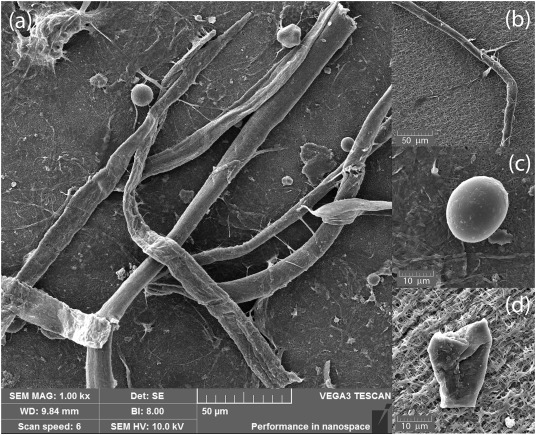
\includegraphics[width=0.5\textwidth]{electronico.jpg}
			\caption{Tamaño de partícula con microscopio electrónico}
		\end{subfigure}
		\begin{subfigure}[h]{0.45\textwidth}
		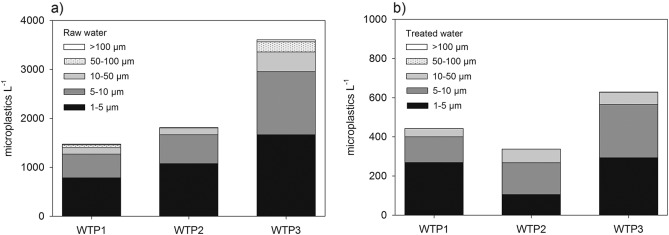
\includegraphics[width=1.2\textwidth]{size.jpg}
		\caption{Distribución de tamaño en agua libre y en agua tratada en las diferentes plantas de tratamientos}
		\end{subfigure}
		
	\end{figure}
	
	\begin{figure}[t!]
		\centering
		\begin{subfigure}[h]{0.45\textwidth}
			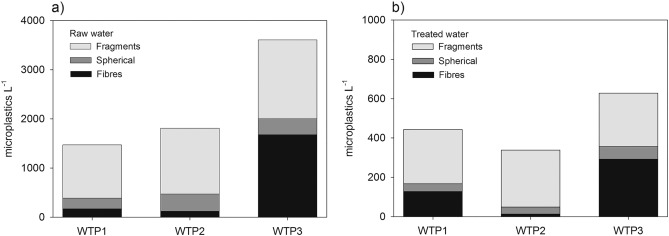
\includegraphics[width=1\textwidth]{proporcion.jpg}
			\caption{Proporciones de los diferentes MPs en agua sin tratar(a) y tratada(b)}
		\end{subfigure}
		\begin{subfigure}[h]{0.45\textwidth}
			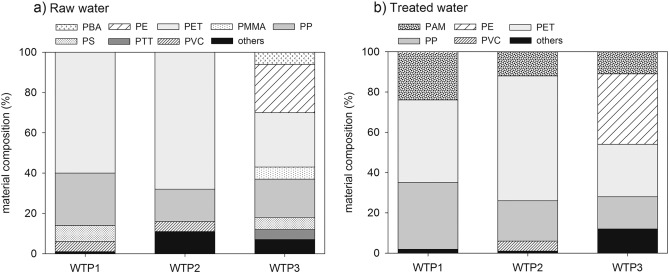
\includegraphics[width=1\textwidth]{composicion.jpg}
			\caption{Composición de de las partículas en agua sin tratar(a) y tratada(b)}
		\end{subfigure}
		
	\end{figure}
	
\end{document}